\documentclass[11pt]{report}

%%  The file ``gmudissertation.sty''  is the GMU latex style file and
%%   should be placed in the same directory as your LaTeX files
\usepackage{gmudissertation}

%%
%% other packages that need to be loaded
%%
\usepackage[numbers]{natbib} % format citations
\usepackage{graphicx}                    %   for imported graphics
\usepackage{amsmath,amssymb,amsthm} %math support
\usepackage{amsfonts}                    %%  for AMS mathematics
\usepackage[normalem]{ulem}              %   a nice standard underline package
\usepackage[noadjust,verbose,sort]{cite} %   arranges reference citations neatly
\usepackage{lscape}                      % to change page orientation
\usepackage{listings}                    % to include source code
\usepackage{color}                       % for colors
\usepackage{float}              % figure placement
%% \usepackage{floatrow}

\usepackage{epstopdf} %covert .eps files to .pdf
\usepackage{curves}
\usepackage{url} %formatting for URL's
\usepackage{setspace} %change line spacing
\usepackage[mathlines]{lineno} %line numbers
\usepackage{relsize} % resize subscripts

\usepackage{tikz,pgfplots} % Creating pictures, images, cartoons, etc...
\usepackage{gnuplot-lua-tikz}
\usepackage{tikz-3dplot}
\usetikzlibrary{arrows,shapes,trees,positioning}
\usetikzlibrary{decorations.markings}
\usetikzlibrary{external} % compile figures separately
\tikzexternalize[prefix=tikz/]
\usetikzlibrary{plotmarks}

\graphicspath{{fig/}} % Location of the graphics files

\usepackage{afterpage}
\usepackage{longtable}
\usepackage[acronym]{glossaries} % create abbreviation and nomenclature lists

% decrease white space above and below caption
%% \setlength{\abovecaptionskip}{-1ex}%{-11pt}
%% \setlength{\belowcaptionskip}{-2ex}%{-8pt}


\definecolor{darkorange}{rgb}{0.9,0.3,0.0}

%%------------------------------------------------------------
%%  Abbreviations 
%%------------------------------------------------------------
%% The file ``dissertationabbrev.sty'' is an (optional) personalized file that
%% may contain any and all LaTeX command (re)definitions that will be used
%% throughout the document
\usepackage{dissertationabbrev}

%%------------------------------------------------------------
%%  Glossary
%%------------------------------------------------------------

%%------------------------------------------------------------
%%  Abbreviations
%%------------------------------------------------------------

\newacronym{aos}{AoS}{array of structures}
\newacronym{cd}{CD}{contact discontinuity}
\newacronym{clf}{CLF}{Courant-Friedrichs-Lewy}
\newacronym{ctu}{CTU}{corner transport upwind}
\newacronym{ct}{CT}{constrained transport}
\newacronym{cuda}{CUDA}{compute unified device architecture}
\newacronym{fcw}{FCW}{fast compound wave}
\newacronym{flops}{FLOPS}{floating-point operations per second}
\newacronym{fr}{FR}{fast rarefaction}
\newacronym{fs}{FS}{fast shocks}
\newacronym{fct}{FCT}{flux corrected transport}
\newacronym{fv}{FV}{finite volume}
\newacronym{gpu}{GPU}{graphics processing unit}
\newacronym{hd}{HD}{hydrodynamics}
\newacronym{hlle}{HLLE}{Harden-Lax-van Leer-Einfeldt}
\newacronym{hllc}{HLLC}{Harden-Lax-van Leer-Contact}
\newacronym{hlld}{HLLD}{Harden-Lax-van Leer-Discontinuities}
\newacronym{ivp}{IVP}{initial value problem}
\newacronym{is}{IS}{intermediate shocks}
\newacronym{mhd}{MHD}{magnetohydrodynamics}
\newacronym{ppm}{PPM}{piece-wise parabolic method}
\newacronym{omp}{OMP}{OpenMP}
\newacronym{rmse}{RMSE}{root-mean-square-error}
\newacronym{rd}{RD}{rotational discontinuity}
\newacronym{scw}{SCW}{slow compound wave}
\newacronym{soa}{SoA}{structure of arrays}
\newacronym{sr}{SR}{slow rarefaction}
\newacronym{ss}{SS}{slow shocks}
\newacronym{stl}{STL}{Standard Template Library}
\newacronym{tbb}{TBB}{thread building blocks}
\newacronym{tvd}{TVD}{total variation diminishing}
\newacronym{vl}{VL}{van Leer}

%%------------------------------------------------------------
%% Nomenclature
%%------------------------------------------------------------
\newglossaryentry{a}{
  name = $a$ ,
  description = acoustic speed of sound,
}
%% \newglossaryentry{numofangels}{
%%   name = $N$ ,
%%   description = The number of angels per needle point
%% }
%% \newglossaryentry{areaofneedle}{
%%   name = $A$ ,
%%   description = The area of the needle point
%% }

%% \makeglossaries

%% \makeglossaries % comment out to compile tikz images ///////////////////////////////////////////////
%% to update glossary: uncommented above line
%%                     compile tex document
%%                     run makeglossaries akercher_dissertation

%%------------------------------------------------------------
%%  Listing options
%%------------------------------------------------------------
\lstset{language=C++,
  basicstyle=\footnotesize\ttfamily,
  morekeywords={Point,Vector,PointArray,VectorArray},
  keywordstyle=\color{blue}\ttfamily,
  stringstyle=\color{darkred}\ttfamily,
  commentstyle=\color{darkorange}\ttfamily,
  morecomment=[l][\color{magenta}]{\#},
  breaklines=true,
  tabsize=2,
  lineskip={-1.5pt} % single line spacing
}

%**************************************************************************************************************
\begin{document}

This is a test file to preview figures.


\begin{figure}[htbp] 
\begin{tabular}{ccc}
\resizebox{0.33\linewidth}{!}{\tikzsetnextfilename{coplanar_a_rotation_00032_0002_1}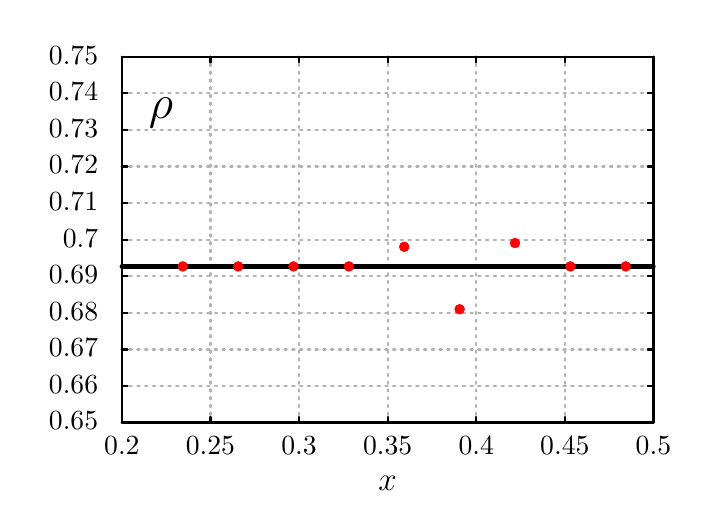
\begin{tikzpicture}[gnuplot]
%% generated with GNUPLOT 4.6p4 (Lua 5.1; terminal rev. 99, script rev. 100)
%% Wed 27 Aug 2014 01:22:14 PM EDT
\path (0.000,0.000) rectangle (8.500,6.000);
\gpfill{rgb color={1.000,1.000,1.000}} (1.196,0.985)--(7.946,0.985)--(7.946,5.630)--(1.196,5.630)--cycle;
\gpcolor{color=gp lt color border}
\gpsetlinetype{gp lt border}
\gpsetlinewidth{1.00}
\draw[gp path] (1.196,0.985)--(1.196,5.630)--(7.946,5.630)--(7.946,0.985)--cycle;
\gpcolor{color=gp lt color axes}
\gpsetlinetype{gp lt axes}
\gpsetlinewidth{2.00}
\draw[gp path] (1.196,0.985)--(7.947,0.985);
\gpcolor{color=gp lt color border}
\gpsetlinetype{gp lt border}
\draw[gp path] (1.196,0.985)--(1.268,0.985);
\draw[gp path] (7.947,0.985)--(7.875,0.985);
\gpcolor{rgb color={0.000,0.000,0.000}}
\node[gp node right,font={\fontsize{10pt}{12pt}\selectfont}] at (1.012,0.985) {0.65};
\gpcolor{color=gp lt color axes}
\gpsetlinetype{gp lt axes}
\draw[gp path] (1.196,1.450)--(7.947,1.450);
\gpcolor{color=gp lt color border}
\gpsetlinetype{gp lt border}
\draw[gp path] (1.196,1.450)--(1.268,1.450);
\draw[gp path] (7.947,1.450)--(7.875,1.450);
\gpcolor{rgb color={0.000,0.000,0.000}}
\node[gp node right,font={\fontsize{10pt}{12pt}\selectfont}] at (1.012,1.450) {0.66};
\gpcolor{color=gp lt color axes}
\gpsetlinetype{gp lt axes}
\draw[gp path] (1.196,1.914)--(7.947,1.914);
\gpcolor{color=gp lt color border}
\gpsetlinetype{gp lt border}
\draw[gp path] (1.196,1.914)--(1.268,1.914);
\draw[gp path] (7.947,1.914)--(7.875,1.914);
\gpcolor{rgb color={0.000,0.000,0.000}}
\node[gp node right,font={\fontsize{10pt}{12pt}\selectfont}] at (1.012,1.914) {0.67};
\gpcolor{color=gp lt color axes}
\gpsetlinetype{gp lt axes}
\draw[gp path] (1.196,2.379)--(7.947,2.379);
\gpcolor{color=gp lt color border}
\gpsetlinetype{gp lt border}
\draw[gp path] (1.196,2.379)--(1.268,2.379);
\draw[gp path] (7.947,2.379)--(7.875,2.379);
\gpcolor{rgb color={0.000,0.000,0.000}}
\node[gp node right,font={\fontsize{10pt}{12pt}\selectfont}] at (1.012,2.379) {0.68};
\gpcolor{color=gp lt color axes}
\gpsetlinetype{gp lt axes}
\draw[gp path] (1.196,2.843)--(7.947,2.843);
\gpcolor{color=gp lt color border}
\gpsetlinetype{gp lt border}
\draw[gp path] (1.196,2.843)--(1.268,2.843);
\draw[gp path] (7.947,2.843)--(7.875,2.843);
\gpcolor{rgb color={0.000,0.000,0.000}}
\node[gp node right,font={\fontsize{10pt}{12pt}\selectfont}] at (1.012,2.843) {0.69};
\gpcolor{color=gp lt color axes}
\gpsetlinetype{gp lt axes}
\draw[gp path] (1.196,3.308)--(7.947,3.308);
\gpcolor{color=gp lt color border}
\gpsetlinetype{gp lt border}
\draw[gp path] (1.196,3.308)--(1.268,3.308);
\draw[gp path] (7.947,3.308)--(7.875,3.308);
\gpcolor{rgb color={0.000,0.000,0.000}}
\node[gp node right,font={\fontsize{10pt}{12pt}\selectfont}] at (1.012,3.308) {0.7};
\gpcolor{color=gp lt color axes}
\gpsetlinetype{gp lt axes}
\draw[gp path] (1.196,3.773)--(7.947,3.773);
\gpcolor{color=gp lt color border}
\gpsetlinetype{gp lt border}
\draw[gp path] (1.196,3.773)--(1.268,3.773);
\draw[gp path] (7.947,3.773)--(7.875,3.773);
\gpcolor{rgb color={0.000,0.000,0.000}}
\node[gp node right,font={\fontsize{10pt}{12pt}\selectfont}] at (1.012,3.773) {0.71};
\gpcolor{color=gp lt color axes}
\gpsetlinetype{gp lt axes}
\draw[gp path] (1.196,4.237)--(7.947,4.237);
\gpcolor{color=gp lt color border}
\gpsetlinetype{gp lt border}
\draw[gp path] (1.196,4.237)--(1.268,4.237);
\draw[gp path] (7.947,4.237)--(7.875,4.237);
\gpcolor{rgb color={0.000,0.000,0.000}}
\node[gp node right,font={\fontsize{10pt}{12pt}\selectfont}] at (1.012,4.237) {0.72};
\gpcolor{color=gp lt color axes}
\gpsetlinetype{gp lt axes}
\draw[gp path] (1.196,4.702)--(7.947,4.702);
\gpcolor{color=gp lt color border}
\gpsetlinetype{gp lt border}
\draw[gp path] (1.196,4.702)--(1.268,4.702);
\draw[gp path] (7.947,4.702)--(7.875,4.702);
\gpcolor{rgb color={0.000,0.000,0.000}}
\node[gp node right,font={\fontsize{10pt}{12pt}\selectfont}] at (1.012,4.702) {0.73};
\gpcolor{color=gp lt color axes}
\gpsetlinetype{gp lt axes}
\draw[gp path] (1.196,5.166)--(7.947,5.166);
\gpcolor{color=gp lt color border}
\gpsetlinetype{gp lt border}
\draw[gp path] (1.196,5.166)--(1.268,5.166);
\draw[gp path] (7.947,5.166)--(7.875,5.166);
\gpcolor{rgb color={0.000,0.000,0.000}}
\node[gp node right,font={\fontsize{10pt}{12pt}\selectfont}] at (1.012,5.166) {0.74};
\gpcolor{color=gp lt color axes}
\gpsetlinetype{gp lt axes}
\draw[gp path] (1.196,5.631)--(7.947,5.631);
\gpcolor{color=gp lt color border}
\gpsetlinetype{gp lt border}
\draw[gp path] (1.196,5.631)--(1.268,5.631);
\draw[gp path] (7.947,5.631)--(7.875,5.631);
\gpcolor{rgb color={0.000,0.000,0.000}}
\node[gp node right,font={\fontsize{10pt}{12pt}\selectfont}] at (1.012,5.631) {0.75};
\gpcolor{color=gp lt color axes}
\gpsetlinetype{gp lt axes}
\draw[gp path] (1.196,0.985)--(1.196,5.631);
\gpcolor{color=gp lt color border}
\gpsetlinetype{gp lt border}
\draw[gp path] (1.196,0.985)--(1.196,1.057);
\draw[gp path] (1.196,5.631)--(1.196,5.559);
\gpcolor{rgb color={0.000,0.000,0.000}}
\node[gp node center,font={\fontsize{10pt}{12pt}\selectfont}] at (1.196,0.677) {0.2};
\gpcolor{color=gp lt color axes}
\gpsetlinetype{gp lt axes}
\draw[gp path] (2.321,0.985)--(2.321,5.631);
\gpcolor{color=gp lt color border}
\gpsetlinetype{gp lt border}
\draw[gp path] (2.321,0.985)--(2.321,1.057);
\draw[gp path] (2.321,5.631)--(2.321,5.559);
\gpcolor{rgb color={0.000,0.000,0.000}}
\node[gp node center,font={\fontsize{10pt}{12pt}\selectfont}] at (2.321,0.677) {0.25};
\gpcolor{color=gp lt color axes}
\gpsetlinetype{gp lt axes}
\draw[gp path] (3.446,0.985)--(3.446,5.631);
\gpcolor{color=gp lt color border}
\gpsetlinetype{gp lt border}
\draw[gp path] (3.446,0.985)--(3.446,1.057);
\draw[gp path] (3.446,5.631)--(3.446,5.559);
\gpcolor{rgb color={0.000,0.000,0.000}}
\node[gp node center,font={\fontsize{10pt}{12pt}\selectfont}] at (3.446,0.677) {0.3};
\gpcolor{color=gp lt color axes}
\gpsetlinetype{gp lt axes}
\draw[gp path] (4.572,0.985)--(4.572,5.631);
\gpcolor{color=gp lt color border}
\gpsetlinetype{gp lt border}
\draw[gp path] (4.572,0.985)--(4.572,1.057);
\draw[gp path] (4.572,5.631)--(4.572,5.559);
\gpcolor{rgb color={0.000,0.000,0.000}}
\node[gp node center,font={\fontsize{10pt}{12pt}\selectfont}] at (4.572,0.677) {0.35};
\gpcolor{color=gp lt color axes}
\gpsetlinetype{gp lt axes}
\draw[gp path] (5.697,0.985)--(5.697,5.631);
\gpcolor{color=gp lt color border}
\gpsetlinetype{gp lt border}
\draw[gp path] (5.697,0.985)--(5.697,1.057);
\draw[gp path] (5.697,5.631)--(5.697,5.559);
\gpcolor{rgb color={0.000,0.000,0.000}}
\node[gp node center,font={\fontsize{10pt}{12pt}\selectfont}] at (5.697,0.677) {0.4};
\gpcolor{color=gp lt color axes}
\gpsetlinetype{gp lt axes}
\draw[gp path] (6.822,0.985)--(6.822,5.631);
\gpcolor{color=gp lt color border}
\gpsetlinetype{gp lt border}
\draw[gp path] (6.822,0.985)--(6.822,1.057);
\draw[gp path] (6.822,5.631)--(6.822,5.559);
\gpcolor{rgb color={0.000,0.000,0.000}}
\node[gp node center,font={\fontsize{10pt}{12pt}\selectfont}] at (6.822,0.677) {0.45};
\gpcolor{color=gp lt color axes}
\gpsetlinetype{gp lt axes}
\draw[gp path] (7.947,0.985)--(7.947,5.631);
\gpcolor{color=gp lt color border}
\gpsetlinetype{gp lt border}
\draw[gp path] (7.947,0.985)--(7.947,1.057);
\draw[gp path] (7.947,5.631)--(7.947,5.559);
\gpcolor{rgb color={0.000,0.000,0.000}}
\node[gp node center,font={\fontsize{10pt}{12pt}\selectfont}] at (7.947,0.677) {0.5};
\gpcolor{color=gp lt color border}
\draw[gp path] (1.196,5.631)--(1.196,0.985)--(7.947,0.985)--(7.947,5.631)--cycle;
\gpcolor{rgb color={0.000,0.000,0.000}}
\node[gp node center,font={\fontsize{10pt}{12pt}\selectfont}] at (4.571,0.215) {\large $x$};
\gpsetlinetype{gp lt plot 0}
\gpsetlinewidth{4.00}
\draw[gp path] (1.196,2.968)--(5.225,2.968);
\draw[gp path] (5.225,2.968)--(5.384,2.968);
\draw[gp path] (5.384,2.968)--(5.536,2.968);
\draw[gp path] (5.536,2.968)--(6.009,2.968);
\draw[gp path] (6.009,2.968)--(6.482,2.968);
\draw[gp path] (6.482,2.968)--(6.633,2.968);
\draw[gp path] (6.633,2.968)--(6.793,2.968);
\draw[gp path] (6.793,2.968)--(7.947,2.968);
\gpcolor{rgb color={1.000,0.000,0.000}}
\gpsetlinewidth{0.50}
\gpsetpointsize{4.44}
\gppoint{gp mark 7}{(1.970,2.968)}
\gppoint{gp mark 7}{(2.673,2.968)}
\gppoint{gp mark 7}{(3.376,2.968)}
\gppoint{gp mark 7}{(4.079,2.968)}
\gppoint{gp mark 7}{(4.782,3.217)}
\gppoint{gp mark 7}{(5.486,2.424)}
\gppoint{gp mark 7}{(6.189,3.265)}
\gppoint{gp mark 7}{(6.892,2.968)}
\gppoint{gp mark 7}{(7.595,2.968)}
\gpcolor{rgb color={0.000,0.000,0.000}}
\node[gp node left,font={\fontsize{10pt}{12pt}\selectfont}] at (1.421,4.934) {\LARGE $\rho$};
%% coordinates of the plot area
\gpdefrectangularnode{gp plot 1}{\pgfpoint{1.196cm}{0.985cm}}{\pgfpoint{7.947cm}{5.631cm}}
\end{tikzpicture}
%% gnuplot variables
} & 
\resizebox{0.33\linewidth}{!}{\tikzsetnextfilename{coplanar_a_rotation_00032_0002_5}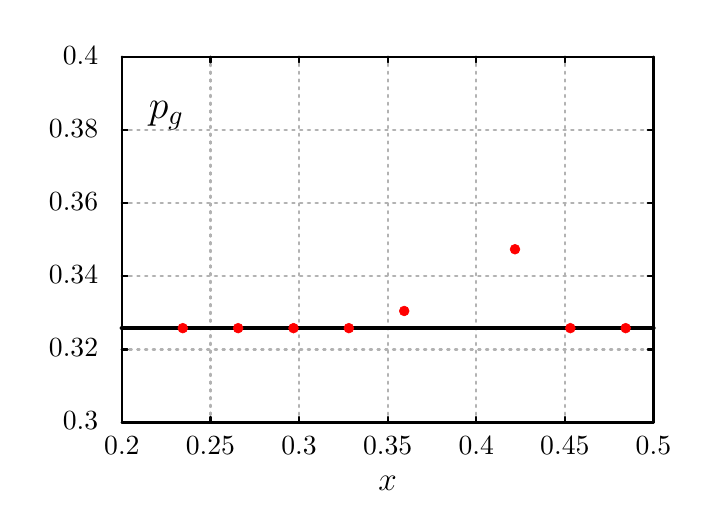
\begin{tikzpicture}[gnuplot]
%% generated with GNUPLOT 4.6p4 (Lua 5.1; terminal rev. 99, script rev. 100)
%% Wed 27 Aug 2014 01:22:14 PM EDT
\path (0.000,0.000) rectangle (8.500,6.000);
\gpfill{rgb color={1.000,1.000,1.000}} (1.196,0.985)--(7.946,0.985)--(7.946,5.630)--(1.196,5.630)--cycle;
\gpcolor{color=gp lt color border}
\gpsetlinetype{gp lt border}
\gpsetlinewidth{1.00}
\draw[gp path] (1.196,0.985)--(1.196,5.630)--(7.946,5.630)--(7.946,0.985)--cycle;
\gpcolor{color=gp lt color axes}
\gpsetlinetype{gp lt axes}
\gpsetlinewidth{2.00}
\draw[gp path] (1.196,0.985)--(7.947,0.985);
\gpcolor{color=gp lt color border}
\gpsetlinetype{gp lt border}
\draw[gp path] (1.196,0.985)--(1.268,0.985);
\draw[gp path] (7.947,0.985)--(7.875,0.985);
\gpcolor{rgb color={0.000,0.000,0.000}}
\node[gp node right,font={\fontsize{10pt}{12pt}\selectfont}] at (1.012,0.985) {0.3};
\gpcolor{color=gp lt color axes}
\gpsetlinetype{gp lt axes}
\draw[gp path] (1.196,1.914)--(7.947,1.914);
\gpcolor{color=gp lt color border}
\gpsetlinetype{gp lt border}
\draw[gp path] (1.196,1.914)--(1.268,1.914);
\draw[gp path] (7.947,1.914)--(7.875,1.914);
\gpcolor{rgb color={0.000,0.000,0.000}}
\node[gp node right,font={\fontsize{10pt}{12pt}\selectfont}] at (1.012,1.914) {0.32};
\gpcolor{color=gp lt color axes}
\gpsetlinetype{gp lt axes}
\draw[gp path] (1.196,2.843)--(7.947,2.843);
\gpcolor{color=gp lt color border}
\gpsetlinetype{gp lt border}
\draw[gp path] (1.196,2.843)--(1.268,2.843);
\draw[gp path] (7.947,2.843)--(7.875,2.843);
\gpcolor{rgb color={0.000,0.000,0.000}}
\node[gp node right,font={\fontsize{10pt}{12pt}\selectfont}] at (1.012,2.843) {0.34};
\gpcolor{color=gp lt color axes}
\gpsetlinetype{gp lt axes}
\draw[gp path] (1.196,3.773)--(7.947,3.773);
\gpcolor{color=gp lt color border}
\gpsetlinetype{gp lt border}
\draw[gp path] (1.196,3.773)--(1.268,3.773);
\draw[gp path] (7.947,3.773)--(7.875,3.773);
\gpcolor{rgb color={0.000,0.000,0.000}}
\node[gp node right,font={\fontsize{10pt}{12pt}\selectfont}] at (1.012,3.773) {0.36};
\gpcolor{color=gp lt color axes}
\gpsetlinetype{gp lt axes}
\draw[gp path] (1.196,4.702)--(7.947,4.702);
\gpcolor{color=gp lt color border}
\gpsetlinetype{gp lt border}
\draw[gp path] (1.196,4.702)--(1.268,4.702);
\draw[gp path] (7.947,4.702)--(7.875,4.702);
\gpcolor{rgb color={0.000,0.000,0.000}}
\node[gp node right,font={\fontsize{10pt}{12pt}\selectfont}] at (1.012,4.702) {0.38};
\gpcolor{color=gp lt color axes}
\gpsetlinetype{gp lt axes}
\draw[gp path] (1.196,5.631)--(7.947,5.631);
\gpcolor{color=gp lt color border}
\gpsetlinetype{gp lt border}
\draw[gp path] (1.196,5.631)--(1.268,5.631);
\draw[gp path] (7.947,5.631)--(7.875,5.631);
\gpcolor{rgb color={0.000,0.000,0.000}}
\node[gp node right,font={\fontsize{10pt}{12pt}\selectfont}] at (1.012,5.631) {0.4};
\gpcolor{color=gp lt color axes}
\gpsetlinetype{gp lt axes}
\draw[gp path] (1.196,0.985)--(1.196,5.631);
\gpcolor{color=gp lt color border}
\gpsetlinetype{gp lt border}
\draw[gp path] (1.196,0.985)--(1.196,1.057);
\draw[gp path] (1.196,5.631)--(1.196,5.559);
\gpcolor{rgb color={0.000,0.000,0.000}}
\node[gp node center,font={\fontsize{10pt}{12pt}\selectfont}] at (1.196,0.677) {0.2};
\gpcolor{color=gp lt color axes}
\gpsetlinetype{gp lt axes}
\draw[gp path] (2.321,0.985)--(2.321,5.631);
\gpcolor{color=gp lt color border}
\gpsetlinetype{gp lt border}
\draw[gp path] (2.321,0.985)--(2.321,1.057);
\draw[gp path] (2.321,5.631)--(2.321,5.559);
\gpcolor{rgb color={0.000,0.000,0.000}}
\node[gp node center,font={\fontsize{10pt}{12pt}\selectfont}] at (2.321,0.677) {0.25};
\gpcolor{color=gp lt color axes}
\gpsetlinetype{gp lt axes}
\draw[gp path] (3.446,0.985)--(3.446,5.631);
\gpcolor{color=gp lt color border}
\gpsetlinetype{gp lt border}
\draw[gp path] (3.446,0.985)--(3.446,1.057);
\draw[gp path] (3.446,5.631)--(3.446,5.559);
\gpcolor{rgb color={0.000,0.000,0.000}}
\node[gp node center,font={\fontsize{10pt}{12pt}\selectfont}] at (3.446,0.677) {0.3};
\gpcolor{color=gp lt color axes}
\gpsetlinetype{gp lt axes}
\draw[gp path] (4.572,0.985)--(4.572,5.631);
\gpcolor{color=gp lt color border}
\gpsetlinetype{gp lt border}
\draw[gp path] (4.572,0.985)--(4.572,1.057);
\draw[gp path] (4.572,5.631)--(4.572,5.559);
\gpcolor{rgb color={0.000,0.000,0.000}}
\node[gp node center,font={\fontsize{10pt}{12pt}\selectfont}] at (4.572,0.677) {0.35};
\gpcolor{color=gp lt color axes}
\gpsetlinetype{gp lt axes}
\draw[gp path] (5.697,0.985)--(5.697,5.631);
\gpcolor{color=gp lt color border}
\gpsetlinetype{gp lt border}
\draw[gp path] (5.697,0.985)--(5.697,1.057);
\draw[gp path] (5.697,5.631)--(5.697,5.559);
\gpcolor{rgb color={0.000,0.000,0.000}}
\node[gp node center,font={\fontsize{10pt}{12pt}\selectfont}] at (5.697,0.677) {0.4};
\gpcolor{color=gp lt color axes}
\gpsetlinetype{gp lt axes}
\draw[gp path] (6.822,0.985)--(6.822,5.631);
\gpcolor{color=gp lt color border}
\gpsetlinetype{gp lt border}
\draw[gp path] (6.822,0.985)--(6.822,1.057);
\draw[gp path] (6.822,5.631)--(6.822,5.559);
\gpcolor{rgb color={0.000,0.000,0.000}}
\node[gp node center,font={\fontsize{10pt}{12pt}\selectfont}] at (6.822,0.677) {0.45};
\gpcolor{color=gp lt color axes}
\gpsetlinetype{gp lt axes}
\draw[gp path] (7.947,0.985)--(7.947,5.631);
\gpcolor{color=gp lt color border}
\gpsetlinetype{gp lt border}
\draw[gp path] (7.947,0.985)--(7.947,1.057);
\draw[gp path] (7.947,5.631)--(7.947,5.559);
\gpcolor{rgb color={0.000,0.000,0.000}}
\node[gp node center,font={\fontsize{10pt}{12pt}\selectfont}] at (7.947,0.677) {0.5};
\gpcolor{color=gp lt color border}
\draw[gp path] (1.196,5.631)--(1.196,0.985)--(7.947,0.985)--(7.947,5.631)--cycle;
\gpcolor{rgb color={0.000,0.000,0.000}}
\node[gp node center,font={\fontsize{10pt}{12pt}\selectfont}] at (4.571,0.215) {\large $x$};
\gpsetlinetype{gp lt plot 0}
\gpsetlinewidth{4.00}
\draw[gp path] (1.196,2.184)--(5.225,2.184);
\draw[gp path] (5.225,2.184)--(5.384,2.184);
\draw[gp path] (5.384,2.184)--(5.536,2.184);
\draw[gp path] (5.536,2.184)--(6.009,2.184);
\draw[gp path] (6.009,2.184)--(6.482,2.184);
\draw[gp path] (6.482,2.184)--(6.633,2.184);
\draw[gp path] (6.633,2.184)--(6.793,2.184);
\draw[gp path] (6.793,2.184)--(7.947,2.184);
\gpcolor{rgb color={1.000,0.000,0.000}}
\gpsetlinewidth{0.50}
\gpsetpointsize{4.44}
\gppoint{gp mark 7}{(1.970,2.184)}
\gppoint{gp mark 7}{(2.673,2.184)}
\gppoint{gp mark 7}{(3.376,2.184)}
\gppoint{gp mark 7}{(4.079,2.184)}
\gppoint{gp mark 7}{(4.782,2.402)}
\gppoint{gp mark 7}{(6.189,3.186)}
\gppoint{gp mark 7}{(6.892,2.184)}
\gppoint{gp mark 7}{(7.595,2.184)}
\gpcolor{rgb color={0.000,0.000,0.000}}
\node[gp node left,font={\fontsize{10pt}{12pt}\selectfont}] at (1.421,4.934) {\Large $p_g$};
%% coordinates of the plot area
\gpdefrectangularnode{gp plot 1}{\pgfpoint{1.196cm}{0.985cm}}{\pgfpoint{7.947cm}{5.631cm}}
\end{tikzpicture}
%% gnuplot variables
} & 
\resizebox{0.33\linewidth}{!}{\tikzsetnextfilename{coplanar_a_rotation_00032_0002_6}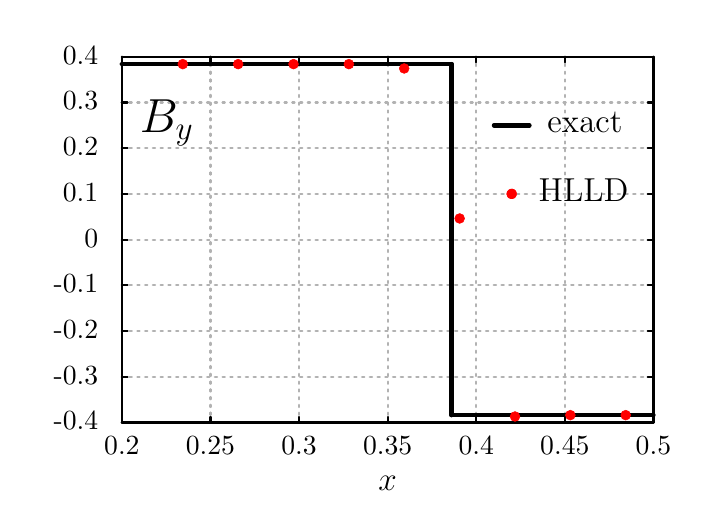
\begin{tikzpicture}[gnuplot]
%% generated with GNUPLOT 4.6p4 (Lua 5.1; terminal rev. 99, script rev. 100)
%% Wed 27 Aug 2014 01:22:14 PM EDT
\path (0.000,0.000) rectangle (8.500,6.000);
\gpfill{rgb color={1.000,1.000,1.000}} (1.196,0.985)--(7.946,0.985)--(7.946,5.630)--(1.196,5.630)--cycle;
\gpcolor{color=gp lt color border}
\gpsetlinetype{gp lt border}
\gpsetlinewidth{1.00}
\draw[gp path] (1.196,0.985)--(1.196,5.630)--(7.946,5.630)--(7.946,0.985)--cycle;
\gpcolor{color=gp lt color axes}
\gpsetlinetype{gp lt axes}
\gpsetlinewidth{2.00}
\draw[gp path] (1.196,0.985)--(7.947,0.985);
\gpcolor{color=gp lt color border}
\gpsetlinetype{gp lt border}
\draw[gp path] (1.196,0.985)--(1.268,0.985);
\draw[gp path] (7.947,0.985)--(7.875,0.985);
\gpcolor{rgb color={0.000,0.000,0.000}}
\node[gp node right,font={\fontsize{10pt}{12pt}\selectfont}] at (1.012,0.985) {-0.4};
\gpcolor{color=gp lt color axes}
\gpsetlinetype{gp lt axes}
\draw[gp path] (1.196,1.566)--(7.947,1.566);
\gpcolor{color=gp lt color border}
\gpsetlinetype{gp lt border}
\draw[gp path] (1.196,1.566)--(1.268,1.566);
\draw[gp path] (7.947,1.566)--(7.875,1.566);
\gpcolor{rgb color={0.000,0.000,0.000}}
\node[gp node right,font={\fontsize{10pt}{12pt}\selectfont}] at (1.012,1.566) {-0.3};
\gpcolor{color=gp lt color axes}
\gpsetlinetype{gp lt axes}
\draw[gp path] (1.196,2.147)--(7.947,2.147);
\gpcolor{color=gp lt color border}
\gpsetlinetype{gp lt border}
\draw[gp path] (1.196,2.147)--(1.268,2.147);
\draw[gp path] (7.947,2.147)--(7.875,2.147);
\gpcolor{rgb color={0.000,0.000,0.000}}
\node[gp node right,font={\fontsize{10pt}{12pt}\selectfont}] at (1.012,2.147) {-0.2};
\gpcolor{color=gp lt color axes}
\gpsetlinetype{gp lt axes}
\draw[gp path] (1.196,2.727)--(7.947,2.727);
\gpcolor{color=gp lt color border}
\gpsetlinetype{gp lt border}
\draw[gp path] (1.196,2.727)--(1.268,2.727);
\draw[gp path] (7.947,2.727)--(7.875,2.727);
\gpcolor{rgb color={0.000,0.000,0.000}}
\node[gp node right,font={\fontsize{10pt}{12pt}\selectfont}] at (1.012,2.727) {-0.1};
\gpcolor{color=gp lt color axes}
\gpsetlinetype{gp lt axes}
\draw[gp path] (1.196,3.308)--(7.947,3.308);
\gpcolor{color=gp lt color border}
\gpsetlinetype{gp lt border}
\draw[gp path] (1.196,3.308)--(1.268,3.308);
\draw[gp path] (7.947,3.308)--(7.875,3.308);
\gpcolor{rgb color={0.000,0.000,0.000}}
\node[gp node right,font={\fontsize{10pt}{12pt}\selectfont}] at (1.012,3.308) {0};
\gpcolor{color=gp lt color axes}
\gpsetlinetype{gp lt axes}
\draw[gp path] (1.196,3.889)--(7.947,3.889);
\gpcolor{color=gp lt color border}
\gpsetlinetype{gp lt border}
\draw[gp path] (1.196,3.889)--(1.268,3.889);
\draw[gp path] (7.947,3.889)--(7.875,3.889);
\gpcolor{rgb color={0.000,0.000,0.000}}
\node[gp node right,font={\fontsize{10pt}{12pt}\selectfont}] at (1.012,3.889) {0.1};
\gpcolor{color=gp lt color axes}
\gpsetlinetype{gp lt axes}
\draw[gp path] (1.196,4.470)--(7.947,4.470);
\gpcolor{color=gp lt color border}
\gpsetlinetype{gp lt border}
\draw[gp path] (1.196,4.470)--(1.268,4.470);
\draw[gp path] (7.947,4.470)--(7.875,4.470);
\gpcolor{rgb color={0.000,0.000,0.000}}
\node[gp node right,font={\fontsize{10pt}{12pt}\selectfont}] at (1.012,4.470) {0.2};
\gpcolor{color=gp lt color axes}
\gpsetlinetype{gp lt axes}
\draw[gp path] (1.196,5.050)--(7.947,5.050);
\gpcolor{color=gp lt color border}
\gpsetlinetype{gp lt border}
\draw[gp path] (1.196,5.050)--(1.268,5.050);
\draw[gp path] (7.947,5.050)--(7.875,5.050);
\gpcolor{rgb color={0.000,0.000,0.000}}
\node[gp node right,font={\fontsize{10pt}{12pt}\selectfont}] at (1.012,5.050) {0.3};
\gpcolor{color=gp lt color axes}
\gpsetlinetype{gp lt axes}
\draw[gp path] (1.196,5.631)--(7.947,5.631);
\gpcolor{color=gp lt color border}
\gpsetlinetype{gp lt border}
\draw[gp path] (1.196,5.631)--(1.268,5.631);
\draw[gp path] (7.947,5.631)--(7.875,5.631);
\gpcolor{rgb color={0.000,0.000,0.000}}
\node[gp node right,font={\fontsize{10pt}{12pt}\selectfont}] at (1.012,5.631) {0.4};
\gpcolor{color=gp lt color axes}
\gpsetlinetype{gp lt axes}
\draw[gp path] (1.196,0.985)--(1.196,5.631);
\gpcolor{color=gp lt color border}
\gpsetlinetype{gp lt border}
\draw[gp path] (1.196,0.985)--(1.196,1.057);
\draw[gp path] (1.196,5.631)--(1.196,5.559);
\gpcolor{rgb color={0.000,0.000,0.000}}
\node[gp node center,font={\fontsize{10pt}{12pt}\selectfont}] at (1.196,0.677) {0.2};
\gpcolor{color=gp lt color axes}
\gpsetlinetype{gp lt axes}
\draw[gp path] (2.321,0.985)--(2.321,5.631);
\gpcolor{color=gp lt color border}
\gpsetlinetype{gp lt border}
\draw[gp path] (2.321,0.985)--(2.321,1.057);
\draw[gp path] (2.321,5.631)--(2.321,5.559);
\gpcolor{rgb color={0.000,0.000,0.000}}
\node[gp node center,font={\fontsize{10pt}{12pt}\selectfont}] at (2.321,0.677) {0.25};
\gpcolor{color=gp lt color axes}
\gpsetlinetype{gp lt axes}
\draw[gp path] (3.446,0.985)--(3.446,5.631);
\gpcolor{color=gp lt color border}
\gpsetlinetype{gp lt border}
\draw[gp path] (3.446,0.985)--(3.446,1.057);
\draw[gp path] (3.446,5.631)--(3.446,5.559);
\gpcolor{rgb color={0.000,0.000,0.000}}
\node[gp node center,font={\fontsize{10pt}{12pt}\selectfont}] at (3.446,0.677) {0.3};
\gpcolor{color=gp lt color axes}
\gpsetlinetype{gp lt axes}
\draw[gp path] (4.572,0.985)--(4.572,5.631);
\gpcolor{color=gp lt color border}
\gpsetlinetype{gp lt border}
\draw[gp path] (4.572,0.985)--(4.572,1.057);
\draw[gp path] (4.572,5.631)--(4.572,5.559);
\gpcolor{rgb color={0.000,0.000,0.000}}
\node[gp node center,font={\fontsize{10pt}{12pt}\selectfont}] at (4.572,0.677) {0.35};
\gpcolor{color=gp lt color axes}
\gpsetlinetype{gp lt axes}
\draw[gp path] (5.697,0.985)--(5.697,5.631);
\gpcolor{color=gp lt color border}
\gpsetlinetype{gp lt border}
\draw[gp path] (5.697,0.985)--(5.697,1.057);
\draw[gp path] (5.697,5.631)--(5.697,5.559);
\gpcolor{rgb color={0.000,0.000,0.000}}
\node[gp node center,font={\fontsize{10pt}{12pt}\selectfont}] at (5.697,0.677) {0.4};
\gpcolor{color=gp lt color axes}
\gpsetlinetype{gp lt axes}
\draw[gp path] (6.822,0.985)--(6.822,5.631);
\gpcolor{color=gp lt color border}
\gpsetlinetype{gp lt border}
\draw[gp path] (6.822,0.985)--(6.822,1.057);
\draw[gp path] (6.822,5.631)--(6.822,5.559);
\gpcolor{rgb color={0.000,0.000,0.000}}
\node[gp node center,font={\fontsize{10pt}{12pt}\selectfont}] at (6.822,0.677) {0.45};
\gpcolor{color=gp lt color axes}
\gpsetlinetype{gp lt axes}
\draw[gp path] (7.947,0.985)--(7.947,5.631);
\gpcolor{color=gp lt color border}
\gpsetlinetype{gp lt border}
\draw[gp path] (7.947,0.985)--(7.947,1.057);
\draw[gp path] (7.947,5.631)--(7.947,5.559);
\gpcolor{rgb color={0.000,0.000,0.000}}
\node[gp node center,font={\fontsize{10pt}{12pt}\selectfont}] at (7.947,0.677) {0.5};
\gpcolor{color=gp lt color border}
\draw[gp path] (1.196,5.631)--(1.196,0.985)--(7.947,0.985)--(7.947,5.631)--cycle;
\gpcolor{rgb color={0.000,0.000,0.000}}
\node[gp node center,font={\fontsize{10pt}{12pt}\selectfont}] at (4.571,0.215) {\large $x$};
\gpsetlinetype{gp lt plot 0}
\gpsetlinewidth{4.00}
\draw[gp path] (1.196,5.537)--(5.225,5.537);
\draw[gp path] (5.225,5.537)--(5.384,5.537);
\draw[gp path] (5.384,1.079)--(5.536,1.079);
\draw[gp path] (5.536,1.079)--(6.009,1.079);
\draw[gp path] (6.009,1.079)--(6.482,1.079);
\draw[gp path] (6.482,1.079)--(6.633,1.079);
\draw[gp path] (6.633,1.079)--(6.793,1.079);
\draw[gp path] (6.793,1.079)--(7.947,1.079);
\draw[gp path] (5.384,5.537)--(5.384,1.079);
\gpcolor{rgb color={1.000,0.000,0.000}}
\gpsetlinewidth{0.50}
\gpsetpointsize{4.44}
\gppoint{gp mark 7}{(1.970,5.537)}
\gppoint{gp mark 7}{(2.673,5.537)}
\gppoint{gp mark 7}{(3.376,5.537)}
\gppoint{gp mark 7}{(4.079,5.537)}
\gppoint{gp mark 7}{(4.782,5.482)}
\gppoint{gp mark 7}{(5.486,3.577)}
\gppoint{gp mark 7}{(6.189,1.062)}
\gppoint{gp mark 7}{(6.892,1.079)}
\gppoint{gp mark 7}{(7.595,1.079)}
\gpcolor{rgb color={0.000,0.000,0.000}}
\gpsetlinewidth{4.00}
\draw[gp path] (5.922,4.760)--(6.372,4.760);
\gpcolor{rgb color={1.000,0.000,0.000}}
\gpsetpointsize{2.67}
\gppoint{gp mark 7}{(6.147,3.889)}
\gppoint{gp mark 7}{(6.147,3.889)}
\gpcolor{rgb color={0.000,0.000,0.000}}
\node[gp node left,font={\fontsize{10pt}{12pt}\selectfont}] at (1.309,4.760) {\LARGE $B_y$};
\node[gp node left,font={\fontsize{10pt}{12pt}\selectfont}] at (6.484,4.760) {\large exact};
\node[gp node left,font={\fontsize{10pt}{12pt}\selectfont}] at (6.372,3.889) {\large HLLD};
%% coordinates of the plot area
\gpdefrectangularnode{gp plot 1}{\pgfpoint{1.196cm}{0.985cm}}{\pgfpoint{7.947cm}{5.631cm}}
\end{tikzpicture}
%% gnuplot variables
} 
%% \tikzsetnextfilename{coplanar_a_rotation_00032_0000_1}
%% 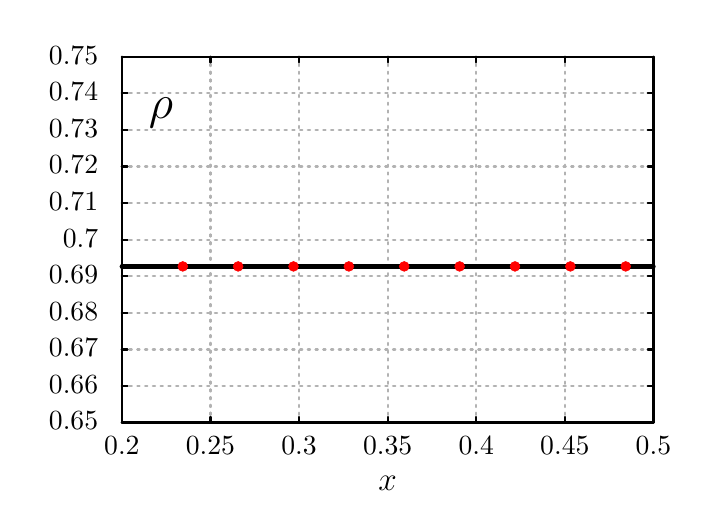
\begin{tikzpicture}[gnuplot]
%% generated with GNUPLOT 4.6p4 (Lua 5.1; terminal rev. 99, script rev. 100)
%% Wed 27 Aug 2014 01:22:11 PM EDT
\path (0.000,0.000) rectangle (8.500,6.000);
\gpfill{rgb color={1.000,1.000,1.000}} (1.196,0.985)--(7.946,0.985)--(7.946,5.630)--(1.196,5.630)--cycle;
\gpcolor{color=gp lt color border}
\gpsetlinetype{gp lt border}
\gpsetlinewidth{1.00}
\draw[gp path] (1.196,0.985)--(1.196,5.630)--(7.946,5.630)--(7.946,0.985)--cycle;
\gpcolor{color=gp lt color axes}
\gpsetlinetype{gp lt axes}
\gpsetlinewidth{2.00}
\draw[gp path] (1.196,0.985)--(7.947,0.985);
\gpcolor{color=gp lt color border}
\gpsetlinetype{gp lt border}
\draw[gp path] (1.196,0.985)--(1.268,0.985);
\draw[gp path] (7.947,0.985)--(7.875,0.985);
\gpcolor{rgb color={0.000,0.000,0.000}}
\node[gp node right,font={\fontsize{10pt}{12pt}\selectfont}] at (1.012,0.985) {0.65};
\gpcolor{color=gp lt color axes}
\gpsetlinetype{gp lt axes}
\draw[gp path] (1.196,1.450)--(7.947,1.450);
\gpcolor{color=gp lt color border}
\gpsetlinetype{gp lt border}
\draw[gp path] (1.196,1.450)--(1.268,1.450);
\draw[gp path] (7.947,1.450)--(7.875,1.450);
\gpcolor{rgb color={0.000,0.000,0.000}}
\node[gp node right,font={\fontsize{10pt}{12pt}\selectfont}] at (1.012,1.450) {0.66};
\gpcolor{color=gp lt color axes}
\gpsetlinetype{gp lt axes}
\draw[gp path] (1.196,1.914)--(7.947,1.914);
\gpcolor{color=gp lt color border}
\gpsetlinetype{gp lt border}
\draw[gp path] (1.196,1.914)--(1.268,1.914);
\draw[gp path] (7.947,1.914)--(7.875,1.914);
\gpcolor{rgb color={0.000,0.000,0.000}}
\node[gp node right,font={\fontsize{10pt}{12pt}\selectfont}] at (1.012,1.914) {0.67};
\gpcolor{color=gp lt color axes}
\gpsetlinetype{gp lt axes}
\draw[gp path] (1.196,2.379)--(7.947,2.379);
\gpcolor{color=gp lt color border}
\gpsetlinetype{gp lt border}
\draw[gp path] (1.196,2.379)--(1.268,2.379);
\draw[gp path] (7.947,2.379)--(7.875,2.379);
\gpcolor{rgb color={0.000,0.000,0.000}}
\node[gp node right,font={\fontsize{10pt}{12pt}\selectfont}] at (1.012,2.379) {0.68};
\gpcolor{color=gp lt color axes}
\gpsetlinetype{gp lt axes}
\draw[gp path] (1.196,2.843)--(7.947,2.843);
\gpcolor{color=gp lt color border}
\gpsetlinetype{gp lt border}
\draw[gp path] (1.196,2.843)--(1.268,2.843);
\draw[gp path] (7.947,2.843)--(7.875,2.843);
\gpcolor{rgb color={0.000,0.000,0.000}}
\node[gp node right,font={\fontsize{10pt}{12pt}\selectfont}] at (1.012,2.843) {0.69};
\gpcolor{color=gp lt color axes}
\gpsetlinetype{gp lt axes}
\draw[gp path] (1.196,3.308)--(7.947,3.308);
\gpcolor{color=gp lt color border}
\gpsetlinetype{gp lt border}
\draw[gp path] (1.196,3.308)--(1.268,3.308);
\draw[gp path] (7.947,3.308)--(7.875,3.308);
\gpcolor{rgb color={0.000,0.000,0.000}}
\node[gp node right,font={\fontsize{10pt}{12pt}\selectfont}] at (1.012,3.308) {0.7};
\gpcolor{color=gp lt color axes}
\gpsetlinetype{gp lt axes}
\draw[gp path] (1.196,3.773)--(7.947,3.773);
\gpcolor{color=gp lt color border}
\gpsetlinetype{gp lt border}
\draw[gp path] (1.196,3.773)--(1.268,3.773);
\draw[gp path] (7.947,3.773)--(7.875,3.773);
\gpcolor{rgb color={0.000,0.000,0.000}}
\node[gp node right,font={\fontsize{10pt}{12pt}\selectfont}] at (1.012,3.773) {0.71};
\gpcolor{color=gp lt color axes}
\gpsetlinetype{gp lt axes}
\draw[gp path] (1.196,4.237)--(7.947,4.237);
\gpcolor{color=gp lt color border}
\gpsetlinetype{gp lt border}
\draw[gp path] (1.196,4.237)--(1.268,4.237);
\draw[gp path] (7.947,4.237)--(7.875,4.237);
\gpcolor{rgb color={0.000,0.000,0.000}}
\node[gp node right,font={\fontsize{10pt}{12pt}\selectfont}] at (1.012,4.237) {0.72};
\gpcolor{color=gp lt color axes}
\gpsetlinetype{gp lt axes}
\draw[gp path] (1.196,4.702)--(7.947,4.702);
\gpcolor{color=gp lt color border}
\gpsetlinetype{gp lt border}
\draw[gp path] (1.196,4.702)--(1.268,4.702);
\draw[gp path] (7.947,4.702)--(7.875,4.702);
\gpcolor{rgb color={0.000,0.000,0.000}}
\node[gp node right,font={\fontsize{10pt}{12pt}\selectfont}] at (1.012,4.702) {0.73};
\gpcolor{color=gp lt color axes}
\gpsetlinetype{gp lt axes}
\draw[gp path] (1.196,5.166)--(7.947,5.166);
\gpcolor{color=gp lt color border}
\gpsetlinetype{gp lt border}
\draw[gp path] (1.196,5.166)--(1.268,5.166);
\draw[gp path] (7.947,5.166)--(7.875,5.166);
\gpcolor{rgb color={0.000,0.000,0.000}}
\node[gp node right,font={\fontsize{10pt}{12pt}\selectfont}] at (1.012,5.166) {0.74};
\gpcolor{color=gp lt color axes}
\gpsetlinetype{gp lt axes}
\draw[gp path] (1.196,5.631)--(7.947,5.631);
\gpcolor{color=gp lt color border}
\gpsetlinetype{gp lt border}
\draw[gp path] (1.196,5.631)--(1.268,5.631);
\draw[gp path] (7.947,5.631)--(7.875,5.631);
\gpcolor{rgb color={0.000,0.000,0.000}}
\node[gp node right,font={\fontsize{10pt}{12pt}\selectfont}] at (1.012,5.631) {0.75};
\gpcolor{color=gp lt color axes}
\gpsetlinetype{gp lt axes}
\draw[gp path] (1.196,0.985)--(1.196,5.631);
\gpcolor{color=gp lt color border}
\gpsetlinetype{gp lt border}
\draw[gp path] (1.196,0.985)--(1.196,1.057);
\draw[gp path] (1.196,5.631)--(1.196,5.559);
\gpcolor{rgb color={0.000,0.000,0.000}}
\node[gp node center,font={\fontsize{10pt}{12pt}\selectfont}] at (1.196,0.677) {0.2};
\gpcolor{color=gp lt color axes}
\gpsetlinetype{gp lt axes}
\draw[gp path] (2.321,0.985)--(2.321,5.631);
\gpcolor{color=gp lt color border}
\gpsetlinetype{gp lt border}
\draw[gp path] (2.321,0.985)--(2.321,1.057);
\draw[gp path] (2.321,5.631)--(2.321,5.559);
\gpcolor{rgb color={0.000,0.000,0.000}}
\node[gp node center,font={\fontsize{10pt}{12pt}\selectfont}] at (2.321,0.677) {0.25};
\gpcolor{color=gp lt color axes}
\gpsetlinetype{gp lt axes}
\draw[gp path] (3.446,0.985)--(3.446,5.631);
\gpcolor{color=gp lt color border}
\gpsetlinetype{gp lt border}
\draw[gp path] (3.446,0.985)--(3.446,1.057);
\draw[gp path] (3.446,5.631)--(3.446,5.559);
\gpcolor{rgb color={0.000,0.000,0.000}}
\node[gp node center,font={\fontsize{10pt}{12pt}\selectfont}] at (3.446,0.677) {0.3};
\gpcolor{color=gp lt color axes}
\gpsetlinetype{gp lt axes}
\draw[gp path] (4.572,0.985)--(4.572,5.631);
\gpcolor{color=gp lt color border}
\gpsetlinetype{gp lt border}
\draw[gp path] (4.572,0.985)--(4.572,1.057);
\draw[gp path] (4.572,5.631)--(4.572,5.559);
\gpcolor{rgb color={0.000,0.000,0.000}}
\node[gp node center,font={\fontsize{10pt}{12pt}\selectfont}] at (4.572,0.677) {0.35};
\gpcolor{color=gp lt color axes}
\gpsetlinetype{gp lt axes}
\draw[gp path] (5.697,0.985)--(5.697,5.631);
\gpcolor{color=gp lt color border}
\gpsetlinetype{gp lt border}
\draw[gp path] (5.697,0.985)--(5.697,1.057);
\draw[gp path] (5.697,5.631)--(5.697,5.559);
\gpcolor{rgb color={0.000,0.000,0.000}}
\node[gp node center,font={\fontsize{10pt}{12pt}\selectfont}] at (5.697,0.677) {0.4};
\gpcolor{color=gp lt color axes}
\gpsetlinetype{gp lt axes}
\draw[gp path] (6.822,0.985)--(6.822,5.631);
\gpcolor{color=gp lt color border}
\gpsetlinetype{gp lt border}
\draw[gp path] (6.822,0.985)--(6.822,1.057);
\draw[gp path] (6.822,5.631)--(6.822,5.559);
\gpcolor{rgb color={0.000,0.000,0.000}}
\node[gp node center,font={\fontsize{10pt}{12pt}\selectfont}] at (6.822,0.677) {0.45};
\gpcolor{color=gp lt color axes}
\gpsetlinetype{gp lt axes}
\draw[gp path] (7.947,0.985)--(7.947,5.631);
\gpcolor{color=gp lt color border}
\gpsetlinetype{gp lt border}
\draw[gp path] (7.947,0.985)--(7.947,1.057);
\draw[gp path] (7.947,5.631)--(7.947,5.559);
\gpcolor{rgb color={0.000,0.000,0.000}}
\node[gp node center,font={\fontsize{10pt}{12pt}\selectfont}] at (7.947,0.677) {0.5};
\gpcolor{color=gp lt color border}
\draw[gp path] (1.196,5.631)--(1.196,0.985)--(7.947,0.985)--(7.947,5.631)--cycle;
\gpcolor{rgb color={0.000,0.000,0.000}}
\node[gp node center,font={\fontsize{10pt}{12pt}\selectfont}] at (4.571,0.215) {\large $x$};
\gpsetlinetype{gp lt plot 0}
\gpsetlinewidth{4.00}
\draw[gp path] (1.196,2.968)--(5.697,2.968);
\draw[gp path] (5.697,2.968)--(7.947,2.968);
\gpcolor{rgb color={1.000,0.000,0.000}}
\gpsetlinewidth{0.50}
\gpsetpointsize{4.44}
\gppoint{gp mark 7}{(1.970,2.968)}
\gppoint{gp mark 7}{(2.673,2.968)}
\gppoint{gp mark 7}{(3.376,2.968)}
\gppoint{gp mark 7}{(4.079,2.968)}
\gppoint{gp mark 7}{(4.782,2.968)}
\gppoint{gp mark 7}{(5.486,2.968)}
\gppoint{gp mark 7}{(6.189,2.968)}
\gppoint{gp mark 7}{(6.892,2.968)}
\gppoint{gp mark 7}{(7.595,2.968)}
\gpcolor{rgb color={0.000,0.000,0.000}}
\node[gp node left,font={\fontsize{10pt}{12pt}\selectfont}] at (1.421,4.934) {\LARGE $\rho$};
%% coordinates of the plot area
\gpdefrectangularnode{gp plot 1}{\pgfpoint{1.196cm}{0.985cm}}{\pgfpoint{7.947cm}{5.631cm}}
\end{tikzpicture}
%% gnuplot variables

\end{tabular}
\end{figure}


\end{document}
